\chapter{Methods}

\section{Lusia Violita Aprilian/1164080}
\subsection{Teori}
\begin{enumerate}
\item Random Forest
	\begin{itemize}
	\item Random Forest diperkenalkan dan diselidiki untuk memprediksi aktivitas biologis kategoris atau kategoris suatu senyawa berdasarkan pada deskripsi kuantitatif dari struktur molekul senyawa. Random Forest adalah ensemble dari pohon klasifikasi atau regresi yang tidak ditandai yang dibuat dengan menggunakan sampel bootstrap dari data pelatihan dan pemilihan fitur acak dalam induksi pohon. Prediksi dibuat dengan menggabungkan (suara terbanyak atau rata-rata) prediksi ensemble.
	\item Gambar Random Forest
		\begin{figure}[ht]
		\centering
		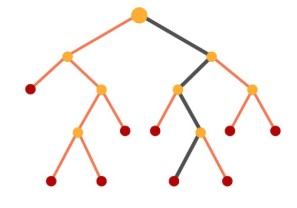
\includegraphics[scale=0.5]{figures/j1.jpg}
		\caption{Random Forest}
		\label{contoh}
		\end{figure}
	\end{itemize}

\item Membaca Dataset
	\begin{itemize}
	\item Berikut adalah cara membaca dataset :
		\begin{enumerate}
			\item Buka Anaconda Navigator lalu jalankan Spyder, kemudian import libraries yang dibutuhkan.
			\item Masukkan kode python untuk membaca file csv, lalu jalankan.
				\begin{figure}[ht]
				\centering
				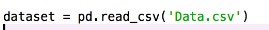
\includegraphics[scale=0.8]{figures/j41.jpg}
				\caption{Kode Python}
				\label{contoh}
				\end{figure}
			\item Maka pada window console akan menampilkan pesan berikut :
				\begin{figure}[ht]
				\centering
				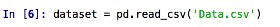
\includegraphics[scale=0.9]{figures/j42.jpg}
				\caption{Pesan Window Console}
				\label{contoh}
				\end{figure}
			\item Dari explorer dapat terlihat dataset yang terimport.
				\begin{figure}[ht]
				\centering
				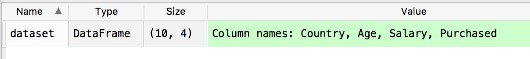
\includegraphics[scale=0.6]{figures/j43.jpg}
				\caption{Dataset}
				\label{contoh}
				\end{figure}
			\item Lalu klik dataset cell, maka akan muncul seperti berikut :
				\begin{figure}[ht]
				\centering
				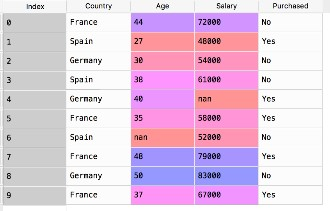
\includegraphics[scale=0.7]{figures/j44.jpg}
				\caption{Hasil Dataset Cell}
				\label{contoh}
				\end{figure}
			\item Seperti yang terlihat pada gambar tersebut dataset ini memiliki Kolom Country, Age, dan Salary sebagai independent variable-nya dan kolom Purchased sebagai dependent variable-nya.
			\item Selanjutnya buat 2 matrix of features yang berisi values dari independent variable dan dependent variable.
			\item Lalu tuliskan perintah berikut :
				\begin{figure}[ht]
				\centering
				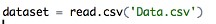
\includegraphics[scale=0.9]{figures/j45.jpg}
				\caption{Perintah}
				\label{contoh}
				\end{figure}
			\item Perintah yang telah dibuat di atas akan membuat sebuah global environment baru dan muncul dataset.
			\item Klikdataset tersebut maka muncul tabel berisi dataset.
		\end{enumerate}
	\end{itemize}

\item Cross Validation
	\begin{itemize}
		\item Cross validation adalah metode statistik yang digunakan untuk memperkirakan keterampilan model pembelajaran mesin. Ini biasanya digunakan dalam pembelajaran mesin yang diterapkan untuk membandingkan dan memilih model untuk masalah pemodelan prediktif yang diberikan karena mudah dipahami, mudah diimplementasikan, dan menghasilkan estimasi keterampilan yang umumnya memiliki bias lebih rendah daripada metode lainnya.
	\end{itemize}
	
\item Menjelaskan Arti Score
	\begin{itemize}
		\item Maksud arti score 44\% pada random forest adalah hasil akurasi.
		\item Maksud arti score 27\% pada decission tree adalah presentasi hasil dari perhitungan dataset.
		\item Maksud arti score 29\% dari SVM adalah hasil pendekatan neural network.
		\item Hasil tersebut didapat dari hasil valdasi silang untuk memastikan bahwa membagi  training test dengan cara yang berbeda. Sehingga didapat outputnya 44\% untuk hutan acak, 27\% untuk pohon keputusan, dan 29\% untuk SVM.
	\end{itemize}

\item Cara Membaca Confusion Matriks
	\begin{itemize}
		\item Mari kita lihat contoh klasifikasi biner berikut ini, yang menunjukkan berapa kali model telah membuat prediksi objek yang benar:
			\begin{figure}[ht]
			\centering
			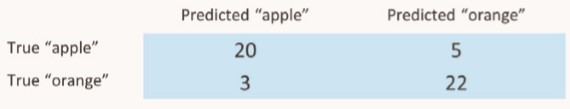
\includegraphics[scale=0.5]{figures/j2a.jpg}
			\caption{Tabel Confusion Matriks}
			\label{contoh}
			\end{figure}
		\item Dalam tabel tersebut, baris apple dan orange mengacu pada kasus di mana objek tersebut sebenarnya sebuah apel atau sebuah jeruk. Kolom merujuk pada prediksi yang dibuat oleh model. Kita melihat bahwa dalam contoh ada 20 apel yang diprediksi dengan benar, sementara ada 5 apel yang salah diidentifikasi sebagai jeruk. Idealnya, confusion matriks harus memiliki semua nilai nol, kecuali untuk diagonal. Di sini kita dapat menghitung akurasi dengan menambahkan angka secara diagonal, sehingga ini semua adalah contoh yang diklasifikasikan dengan benar, dan membagi jumlah tersebut dengan jumlah semua angka dalam matriks:
			\begin{figure}[ht]
			\centering
			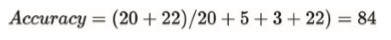
\includegraphics[scale=0.5]{figures/j2b.jpg}
			\caption{Rumus Confusion Matriks}
			\label{contoh}
			\end{figure}
		\item Sehingga dari perhitungan tersebut kita mendapat akurasi 84%.
		\item Berikut adalah gambar klasifikasi biner :
			\begin{figure}[ht]
			\centering
			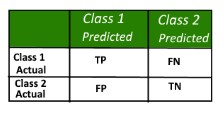
\includegraphics[scale=0.5]{figures/j2c.jpg}
			\caption{Confusion Matriks}
			\label{contoh}
			\end{figure}
	\end{itemize}
	
\item Voting Pada Random Forest
	\begin{itemize}
		\item Voting pada random forest merupakan metode yang paling umum digunakan setelah classifier membuat keputusan.
		\item Gambar voting pada random forest
			\begin{figure}[ht]
			\centering
			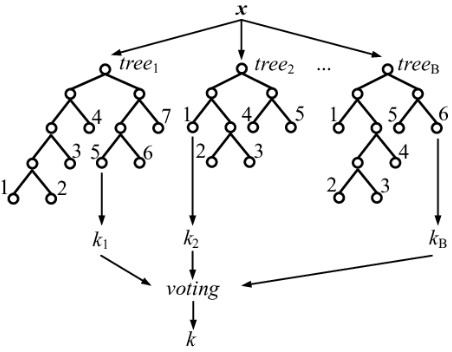
\includegraphics[scale=0.5]{figures/j3.jpg}
			\caption{Voting Pada Random Forest}
			\label{contoh}
			\end{figure}
	\end{itemize}

\end{enumerate}


\section{Rahmi Roza/1164085}
\subsection{Teori}
Penyelesaian Tugas Harian 5 ( No. 1-6 )
\begin{enumerate}
\item Random Forest Dan Ilustrasi Gambarnya
\begin{itemize}
\item Pengertian Random Forest:
\par Random Forest adalah suatu algoritma yang digunakan pada klasifikasi data dalam jumlah yang besar. Klasifikasi random forest dilakukan melalui penggabungan pohon  dengan melakukan training pada sampel data yang dimiliki. Penggunaan pohon (tree) yang semakin banyak akan mempengaruhi akurasi yang akan didapatkan menjadi lebih baik. Penentuan klasifikasi dengan random forest diambil berdasarkan hasil voting dari pohon yang terbentuk. Pemenang dari pohon yang terbentuk ditentukan dengan vote terbanyak. 
\par Pembangunan pohon  pada random forest sampai dengan mencapai ukuran maksimum dari pohon data. Akan tetapi,pembangunan pohon random foresttidak dilakukan pemangkasan  yang merupakan sebuah metode untuk mengurangi kompleksitas ruang.
\item Ilustrasi Gambar Random Forest :
\par

\begin{figure}[ht]
\centering
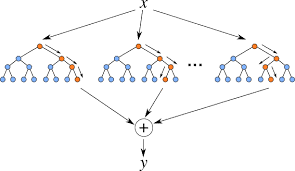
\includegraphics[scale=0.9]{figures/aku1.png}
\caption{Random Forest}
\label{contoh}
\end{figure}

\par
\end{itemize}

\item Cara Membaca Dataset, Dan artikan makna setiap file dan isinya.
\begin{itemize}
\item Cara Membaca Dataset :
\par (a) Buka Anaconda Navigator lalu jalankan Spyder, kemudian import libraries yang dibutuhkan.
\par (b) Masukkan kode python untuk membaca file csv, lalu jalankan.
\begin{figure}[ht]
\centering
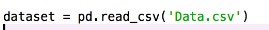
\includegraphics[scale=0.5]{figures/21.jpeg}
\caption{(b)}
\label{contoh}
\end{figure}
\par (c) Maka pada window console akan menampilkan pesan berikut :
\begin{figure}[ht]
\centering
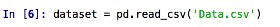
\includegraphics[scale=0.9]{figures/22.jpeg}
\caption{(c)}
\label{contoh}
\end{figure}
\par (d) Dari explorer dapat terlihat dataset yang terimport.
\begin{figure}[ht]
\centering
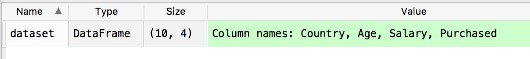
\includegraphics[scale=0.6]{figures/23.jpeg}
\caption{(d)}
\label{contoh}
\end{figure}
\par (e) Lalu klik dataset cell, maka akan muncul seperti berikut :
\begin{figure}[ht]
\centering
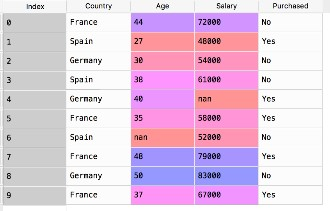
\includegraphics[scale=0.9]{figures/24.jpeg}
\caption{(e)}
\label{contoh}
\end{figure}
\par (f) Seperti yang terlihat pada gambar tersebut dataset ini memiliki Kolom Country, Age, dan Salary sebagai independent variable-nya dan kolom Purchased sebagai dependent variable-nya.
\par (g) Selanjutnya buat 2 matrix of features yang berisi values dari independent variable dan dependent variable.
\par (h) Lalu tuliskan perintah berikut :
\begin{figure}[ht]
\centering
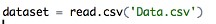
\includegraphics[scale=0.9]{figures/25.jpeg}
\caption{(h)}
\label{contoh}
\end{figure}
\par (i) Perintah yang telah dibuat di atas akan membuat sebuah global environment baru dan muncul dataset.
\par (j) Klik dataset tersebut maka muncul tabel berisi dataset.

\end{itemize}

\item Cross Validation 
\begin{itemize}
\item Pengertian Cross Validation :
\par Cross Validation atau bisa disebut estimasi rotasi ,adalah sebuah teknik validasi model untuk menilai bagaimana hasil statistik analisis akan menggeneralisasi kumpulan data independen. Teknik ini utamanya digunakan untuk melakukan prediksi model dan memperkirakan seberapa akurat sebuah model prediktif ketika dijalankan dalam praktiknya. 
\par Dalam sebuah masalah prediksi, sebuah model biasanya diberikan kumpulan data (dataset) yang diketahui untuk digunakan dalam menjalankan pelatihan (dataset pelatihan), serta kumpulan data yang tidak diketahui (atau data yang pertama kali dilihat) terhadap model yang diuji (pengujian dataset).
\par Tujuan dari validasi silang adalah untuk mendefinisikan dataset untuk "menguji" model dalam tahap pelatihan (yaitu, validasi data), dalam rangka untuk membatasi masalah seperti terjadinya overfitting, memberikan wawasan tentang bagaimana model akan menggeneralisasi independen dataset (yaitu, tidak diketahui dataset, misalnya dari masalah nyata), dll.


\par
\end{itemize}
\item Penjelasan / Maksud Dari Score pada :
\begin{itemize}
\item Random forest ( 44\% )
\par Maksud arti score 44\%  pada random forest adalah hasil dari akurasi. Yang menggunakan 5 buah atribut yaitu dari 5 baris pertama dari set pelatihan yang akan memprediksi spesies 10, 28, 156, 10 dan 43.
\par

\item Decision Tree ( 27\% )
\par Maksud arti score 27\% pada decission tree adalah presentasi hasil dari perhitungan dataset. Dari set tentang burung pipit. Confusion matrix memberi tau hal-hal yang diharapkan, artinya, butrung-burung yang terlihat mirip saling bingung satu sama lain. 
\par

\item SVM ( 29\% )
\par Maksud arti score 29\% dari SVM adalah hasil pendekatan jaringan saraf. Di sini, akurasinya adalah 27\%, yang kurang dari akurasi 44\% sebelumnya. Oleh karena itu, dessicion tree menjadi  lebih buruk. Jika kita menggunakan Support Vector Machine (SVM), yang merupakan neural pendekatan jaringan, outputnya 29\%. Jadi 29\% pada SVM merupakan hasil otputannya.
\par
\par Hasil tersebut didapat dari hasil valdasi silang untuk memastikan bahwa membagi training test dengan cara yang berbeda. Sehingga didapat outputnya 44\% untuk hutan acak, 27\% untuk pohon keputusan, dan 29\% untuk SVM.
\par
\end{itemize}

\par
\item Confusion Matrix Dan Ilustrasinya
\begin{itemize}
\item Cara Membaca Confusion Matrix :
\par Perhitungan confusion matrix adalah sebagai berikut, akan saya beri contoh sederhana yaitu pengambilan keputusan untuk mendapatkan bantuan beasiswa. Saya menggunakan dua atribut, yaitu rekening listrik dan gaji. Yang pertama kita lakukan yaitu mencari 4 nilai yaitu a,b,c, dan d:
\par a= 4
\par b= 1
\par c= 1
\par d= 2
\par Kemudian kita dapat mencari nilai Recall, Precision, accuracy dan Error Rate
\par Recall =2/(1+2) = 0,66
\par  Precision = 2/(1+2) = 0,66
\par Accuracy =(4+2)/(4+1+1+2) = 0,75
\par Error Rate =(1+1)/(4+1+1+4) = 0,2
\par Ilustrasi Confusion Matrix :
\par
\begin{figure}[ht]
\centering
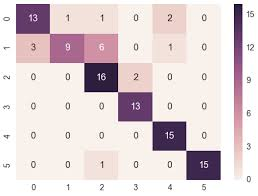
\includegraphics[scale=0.8]{figures/aku3.jpg}
\caption{Confussion Matrik}
\label{contoh}
\end{figure}
\end{itemize}

\par
\par
\item Voting Random Forest Dan Ilustrasi Gambarnya.
\par
\begin{itemize}
\item Pengertian Voting pada Random Forest	:
\par Metode ensemble dapat mencapai akurasi tinggi dengan membangun beberapa pengklasifikasi dan menjalankan
masing-masing secara mandiri. Ketika classifier membuat sebuah keputusan, kamu dapat memanfaatkan yang terbaik
keputusan umum dan rata-rata. Jika kita menggunakan metode yang paling umum, itu disebut voting.
\item Ilustrasi Gambar Voting Random Forest :
\begin{figure}[ht]
\centering
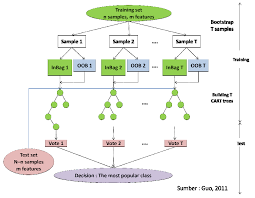
\includegraphics[scale=0.8]{figures/aku2.png}
\caption{Voting Random forest}
\label{contoh}
\end{figure}
\end{itemize}
\end{enumerate}


\end{document}


\section{Method 1}
Definition, steps, algoritm or equation of method 1 and how to apply into your data
\section{Method 2}
Definition, steps, algoritm or equation of method 2 and how to apply into your data